\section{Pragmatics of Model Construction\label{sec:prprac}}
The modelling of the network proposed in section~\ref{sec:bcnetwork}
assumes that all sending and receiving of messages is performed
`perfectly'.  We need now to clarify what we mean by perfect behaviour
in this context and to explain how models can be built which
accommodate the imperfections of the real world.
\subsection{Imperfect Senders}
When transmitting a message, we assume that the
perfect sender will be ready to `announce' its message to the channel,
by entering it into arbitration, at the very instant that it performs the
transition from $\kk!\ii.\xx$. This is not to say that the message will,
in fact, be transmitted at this instant but simply that it would be if the
channel were free and there were no higher priority messages awaiting 
transmission. In reality, it will be necessary for
the sending process to configure a communications controller to transmit
its message. This will require some time for the process to accomplish and
may also require some internal activity on the part of the 
controller following configuration. Our abstraction, however, 
has removed all reference 
to communications controllers and so we must accommodate this behaviour entirely
within a description of the sending process. The configuration time is 
easily accounted for; we simply include a computation to model it:
$[Conf_l, Conf_u] ; \kk!\ii.\xx$, where $Conf_l$ and $Conf_u$ are
the lower and upper bounds, respectively, on the time taken by the process
to configure the communications controller for message transmission.
Accounting for internal controller activity is less straightforward,
but we believe this is a price worth paying to avoid having to model the
controller explicitly. We simply extend the upper bound on the time taken
to configure the controller to allow also for the controller's internal
activity. Of course, this delay will not in fact be experienced by the
configuring process. We can compensate for this by reducing the upper
bound on any following computation (there will certainly be a following
computation, if only to account for the return from the call to
configure the controller) by the same amount. Modelling the queueing
of a message for 
transmission now looks like
\[
[Conf_l, Conf_u + Cint_u] ; \kk!\ii.\xx ; [Next_l, Next_u - Cint_u]
\]
where $Cint_u$ is the upper bound on the controller's internal
activity (we assume a lower bound of 0), and $Next_l, Next_u$ give the
bounds on any following computation. Of course, for this adjustment to
be meaningful, it must be the case that $Next_l \leq Next_u - Cint_u$.
We can illustrate these ideas by reference to~Figure~\ref{fig:impsnd}.

Let $S$ be the process and $T$ be the controller. At point $A$, $S$
begins configuring $T$ to transmit a message. $S$'s part in the configuration
completes somewhere between $B$ and $C$. However, $T$ may not
be properly configured until it completes some internal activity. 
$CD$, being the distance from $C$ to $D$, represents the upper bound on 
the time taken by $T$ to complete its internal activity. The upper bound 
on the configuration is increased to advance its latest possible
completion time to point $D$. Since the delay, $CD$, will not, in fact, be
experienced by $S$, we can also adjust the upper bound on the following
computation to bring back its latest completion time from $G$ to $F$
which is where it would have been without the previous adjustment. The net
effect of these adjustments is include in the model behaviours in 
which configuration completes as late as may occur in an implementation
while not including unnecessary behaviours. 

\begin{figure}
\begin{center}
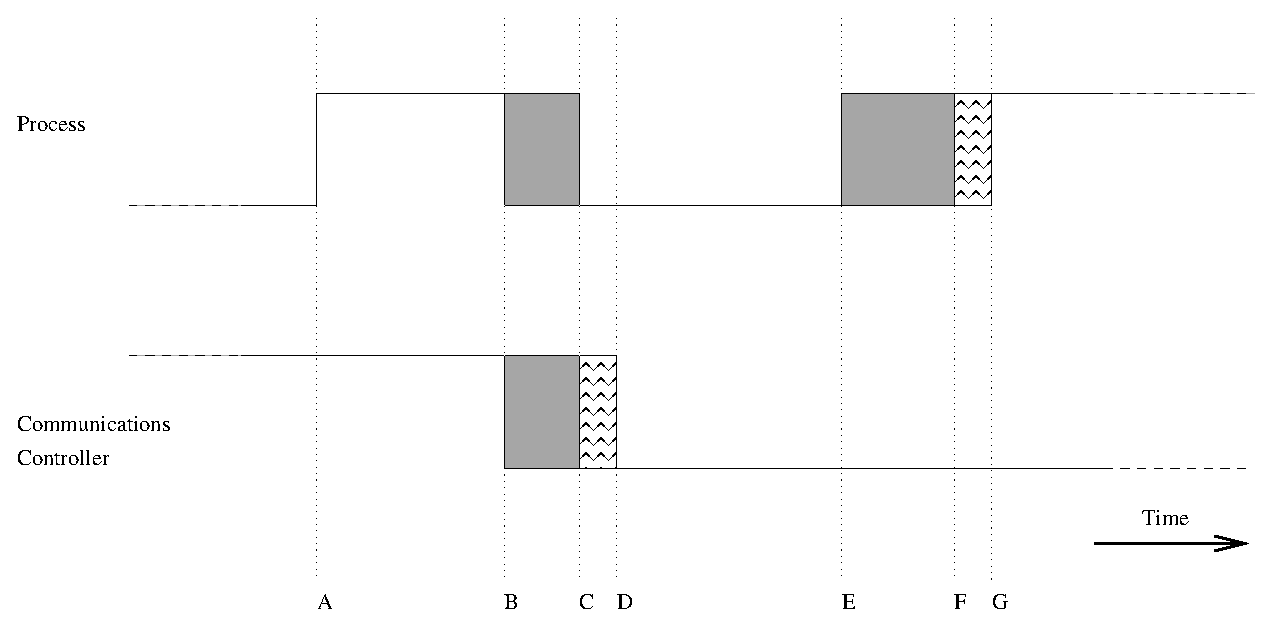
\includegraphics[width=.75\linewidth]{PRACTICE/impsnd.eps}
\end{center}
\caption{Modelling an `imperfect' sender\label{fig:impsnd}}
\end{figure}


\subsection{Imperfect Receivers}
Modelling receivers suffers similar difficulties. A process behaving as
a `perfect' receiver for a message $\mm$ on a channel $\kk$ will 
exhibit the following properties:
\begin{enumerate}
\item It will receive 
any such message which triggers an acceptance test after the process reaches
a state in which a transition from $\kk?\mm$ is an initial action.
\item
Immediately following such a transition, it will have access to the 
transmitted message.
\item
It will {\em not\/} receive any message $\mm'$ on any channel $\kk'$ 
for which a transition from $\kk'?\mm'$ is not
an initial action of the process at the instant of the triggering of the
acceptance test for $\kk'?\mm'$.
\end{enumerate}       

Unfortunately, receivers in the real world exhibit none of these
properties.  Each is confounded by interactions between the receiving
process and its supporting communications controller as described
below.
\begin{enumerate}
\item As with sending, a receiving process must configure a controller
before it can receive a message. Following configuration, the controller
may need to perform some internal activity before it is able to accept
a message for which it has just been configured.
\item Following a successful acceptance test, there will be a delay before
the transmitted data is available to the receiving process. This delay
will include at least the time taken for the controller to raise an 
interrupt signalling message arrival, for the interrupt to be recognised
and for the interrupt handler to transfer the data from the message buffer
into the address space of the receiving process. 
\item The propagation delay of the signal in the transmission medium causes
different controllers to `hear' the acceptance test trigger (ATT) at
different times, depending on their distance from the transmitter. A
perfect receiver suffers no propagation delay and so our model imposes
the requirement that a process which has not configured its controller
(allowing for internal controller activity) by the time at which a
perfect receiver would hear the ATT, will not receive the message. In
practice, receivers will hear the ATT slightly later than the perfect
receiver (bounded by 1 bit time for CAN) and so may accept messages
which the perfect receiver would ignore. We can account for this
behaviour by {\em reducing\/} the lower bound on the configuration
time, thus admitting the possibility that we may receive messages that
would otherwise be missed, and by {\em increasing\/} the upper bound
of the following computation to compensate for the propagation delay
in the timing of the ATT. This is illustrated in
Figure~\ref{fig:imprcv}.  Let $S$ be the process and $T$ be the
channel. At point $A$, $T$ begins carrying a message frame whose
acceptance point will occur somewhere between $C$ and $D$. Meanwhile
at point $B$, $S$ begins configuring its controller to receive
messages of the kind currently being transmitted. $D'$ is the earliest
point at which the configuration can complete. $DD'$, being the
distance from $D$ to $D'$, represents the maximum possible propagation
delay, which, if experienced, allows $S$ to accept the transmitted
message. We adjust the lower bound of the configuration time to bring
its earliest completion time back from $D'$ to $D$, so allowing the
possibility of acceptance. $D'E'$ represents the upper bound on the
time taken to complete the computation, $Comp$, following acceptance.
Since we are modelling an acceptance which actually occurs at $D'$ as
occurring at $D$, we need to adjust the upper bound of $Comp$ to
advance its latest completion time from $E$ to $E'$ where it belongs.
\end{enumerate}
A model of reception which takes account of all of these factors is thus:
\[
[Conf_l - Prop_u, Conf_u + Cint_u] ; \kk?\mm ; [Next_l, Next_u + Prop_u]
\]
where $Conf_l, Conf_u$ are the bounds on the time for the process to configure
the controller, $Prop_u$ is the upper bound on the propagation delay, $Cint_u$
is the upper bound on the controller's internal activity following 
configuration before it will be ready to accept the message for which it has
just been configured and $Next_l, Next_u$ are the bounds on the time required
for the message data to become available to the receiving process. Note that
we make no adjustment to $Next_l$ to allow for propagation delay, since
in general, we can not tell whether the process has experienced such a delay
or not. Nor is it possible to make an adjustment to $Next_u$ to 
compensate for the time taken for internal controller activity, since the
process itself will, in fact, experience this delay, unlike in the case of
sending a message. In this way, it is ensured that the model is a 
conservative abstraction and that the number of additional, unnecessary
behaviours is kept as small as is reasonably possible. 


\begin{figure}
\begin{center}
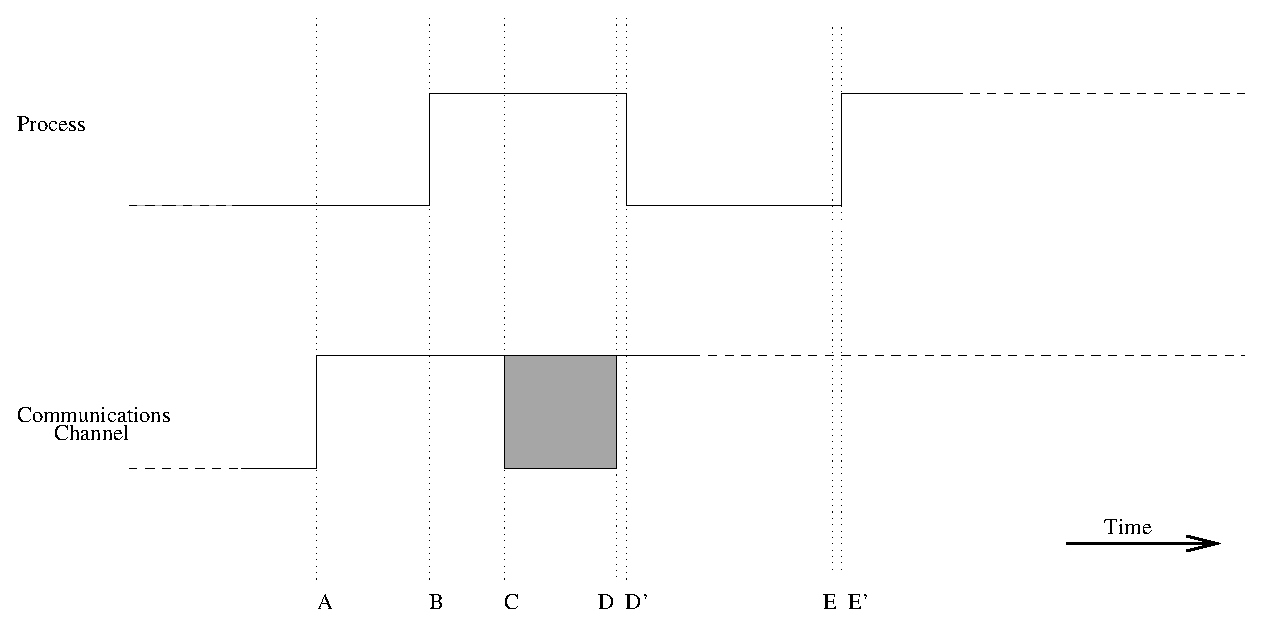
\includegraphics[width=.75\linewidth]{PRACTICE/imprcv.eps}
\caption{Modelling an `imperfect' receiver.\label{fig:imprcv}}
\end{center}
\end{figure}
